%Dokumenteigenschaften
\documentclass[a4paper, 12pt]{article}
%import
\usepackage{blindtext}
\usepackage{hyperref}
\usepackage{pdfpages}
\usepackage{amsmath}
\usepackage{amssymb}
\usepackage[b]{esvect}
\hypersetup{linktoc=all}

\begin{document}
	%Titelseite
	\begin{titlepage}
		\title{\Large{\textbf{\underline{Simulation von Boids nach der Idee von Craig Reynolds}}}}
		\author{Oliver Fritzler}
		\date{\today}
		\maketitle
	\end{titlepage}
	%Inhaltsverzeichnis
	\title{\Large{\textbf{\underline{Inhaltsverzeichnis}}}}
	\tableofcontents
	\newpage
	%Abbildungsverzeichnis
	\section{Abbildungsverzeichnis}
	\newpage
	%Quellennachweis
	\section{Quellennachweis}
	\newpage
	%UML-Diagramm
	\section{UML-Diagramm}
	\includegraphics[scale=0.75, page=2]{UML/Boids_UML.pdf}
	\newpage
	%Grundidee
	\section{Grundidee}
	\subsection{Umgebung}
		Die Programmiersprache \emph{\textbf{Python}} war vorgegeben, die Bibliothek zur grafischen Darstellung war frei überlassen. Aufgrund der eindeutigen und verständlichen Syntax, fiel die Auswahl auf die \emph{\textbf{ursina engine}}, welche auf der \emph{\textbf{panda3D engine}} basiert. Ursina ermöglicht es neben vorgegebenen Modellen auch blender-Dateien als Modelle für die einzelnen Objekte zu verwenden. Diese Objekte werden dargestellt und durch spezifische Funktionen jedes Bild aktualisiert. Dadurch kann man sowohl die Position durch Addition verändern, als auch Eingaben des Benutzers verarbeiten. 
	
	\subsection{Umsetzung des Raumes}
		Um die Darstellung übersichtlich zu machen, erstellt man einen Bereich in denen sich die Boids bewegen könnnen. Dies schafft man, indem man zum Beispiel lange Quader erstellt und diese in Form einer Box anordnet. Somit hat man den Bewegungsraum als Würfel definiert.
		
	\subsection{Umsetzung der Boids}
		Boids sind Körper, aus diesem Grund brauchen sie eine Form. Dafür eignet sie die Form einer Pyramide gut, da diese auch die Ausrichtung der Bewegung zeigen kann. Da diese sich bewegen, haben sie eine Geschwindigkeit für jede einzelne Achse um die Bewegung in drei Dimensionen durchführen zu können. Die Positionsänderung wird jedes Bild durch einfaches addieren der Geschwindigkeit auf einer Achse auf die Position auf der jeweiligen Achse durchgeführt. Die Werte für sowohl Position auch Geschwindigkeit liegen im \textbf{$\mathbb{D}$ $\in$ $\mathbb{Z}$}, da man sowohl eine positive als auch eine negative Geschwindigkeit haben kann und deswegen auch negative Positionen bis zu einem bestimmten Grad haben kann.\linebreak
		
		\textbf{\underline{Verhalten}}
		Das Verhalten der Boids an den Wänden kann man auf verschiedene Weise gestalten. Bei dieser Umsetzung sind 2 davon implementiert worden. Die eine ähnelt dem Ball aus dem Spiel \emph{\textbf{Pong}}. Hierbei bewegt sich der Boid auf eine Wand in einem bestimmten Winkel zu, jedoch wird dieser nach dem "Einfallswinkel = Ausfallswinkel"-Prinzip "gespiegelt" und entfernt sich wieder von der Wand. Dabei muss lediglich einer der Geschwindigkeiten mit der -1 multipliziert werden. Bei der zweiten Umsetzung werden die Boids beim Berühen der einen Wand zur gegenüberliegenden Wand "teleportiert". Dies ist durch Ändern der Positionsvariable auf der jeweiligen Achse möglich.\linebreak
		
		\textbf{\underline{Rotation}} 
		Neben der Bewegung der Boids gehört auch die Ausrichtung zu den Boids. Diese findet statt indem man den Winkel zwischen dem Bewegungsvektor und dem Einheitsvektor der jeweiligen Achse berechnet. Dabei wird die Rotation nicht in 3D berechnet, sondern im 2D um die Rotation zu einer dreidimensionalen zusammenzusetzen. Dies bedeutet, dass man zur Berechnung die Vektoren $\vv{XY}$, $\vv{XZ}$ und $\vv{YZ}$ benutzt.
		Die Formel zur Berechnung lautet, wobei heier $\vec{a}$ einer der zuvor genannten Vektoren ist und $\vec{b}$ einer der drei Einheitsvektoren ist:
		
		\begin{center}
			$\vartheta$ $=$ $\arccos\left(\dfrac{\vec{a}\circ\vec{b}}{\left|\vec{a}\right|\cdot\left|\vec{b}\right|}\right)$
		\end{center}
	
		Das Ergebnis dieser Rechnung wird dann durch Umwandlung in den Winkel umgewandelt, welcher dann von Ursina nach ihrem Rotationsverhalten benutzt werden kann.
	\subsection{Regeln}
	Boids sind Objekte die sich in einem Raum bewegen. Dabei verfolgen sie drei Grundregeln:
	\begin{itemize}
		\item\underline{Seperation}\linebreak
		Diese Regel besagt, dass jeder einzelne Boid versucht, keinen anderen Boid zu treffen. 
		\item\underline{Alignement}\linebreak
		Diese Regel besagt, dass jeder Boid versucht, in die selbe Richtung wie ein anderer sich zu bewegen. Dadurch entsteht ein sogenannter "Flock" also ein Schwarm von Boids.
		\item\underline{Coheseion}\linebreak
		Diese Regel besagt, dass die Boids in die Mitte des Schwarms steuern.
	\end{itemize}
		
	\newpage
	%wichtigste Funktionen
	\section{wichtigste Funktionen}
	\newpage
\end{document}
